\chapter{单用户下的可验证对称加密搜索方案研究}
\label{cha:single-user}
\section{引言}
本章提出了一种普适的可验证对称加密搜索框架\single,该框架可以在单用户场景下工作,与任意对称加密搜索方案结合后,可以为用户提供加密搜索的结果验证服务。本章的主要内容安排如下:首先介绍了单用户场景下的系统框架,介绍了该框架的参与方及其所承担的计算任务;接着,通过一个正式定义从抽象层面介绍了该框架工作的流程和每个参与方涉及到的算法。随后,对\single 框架涉及到的算法进行了详细分析,包括数据持有者构建和更新验证索引的算法,云服务器搜索验证索引并生成结果证明的算法,数据持有者进行结果验证的算法。随后通过一个简单的例子对这几个算法进行了详细的阐述。最后,通过安全性分析和实验结果分析证明\single 方案可以达到设计目标中的安全性要求和性能要求。

\section{系统架构}
单用户场景下的可验证对称加密搜索框架如图~\ref{fig:GS-VSSE}所示,数据持有者即为数据搜索用户本身。初始化时需要数据持有者对自身的数据集进行加密,并对该数据集构建加密的验证索引,用于后续结果验证。数据持有者将加密文件集和验证索引上传给云服务器存储,并在需要时更新数据集和验证索引。当用户需要进行关键字搜索时,他将会构建出一个与关键字相关的搜索令牌,提交给云服务器进行搜索。云服务器接收到该搜索令牌后,通过某个加密搜索方案取得加密搜索结果,同时通过搜索验证索引取得一个结果证明,将加密搜索结果和结果证明返回给用户。用户在收到搜索结果和结果证明后,对其进行结果验证,若验证失败,则丢弃该结果。
\begin{figure}[t]
\centering
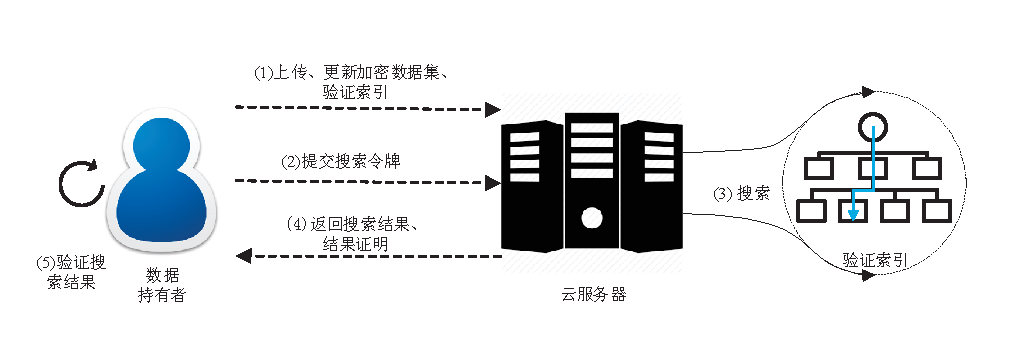
\includegraphics[width=6 in]{fig/GS-VSSE}
\DeclareGraphicsExtensions.
\caption{单用户场景下的可验证对称加密搜索框架\single}
\label{fig:GS-VSSE}
\end{figure}

\section{方案流程}

\begin{definition}[\textbf{\single 方案}]\label{def:single}
  {\itshape
      在\single 方案中,参与方有两个,分别为数据持有者本身和不可信的云服务器。数据持有者向云服务器提供加密数据集和验证索引,使得云服务器在用户搜索时可以向其返回结果证明,用于确保加密搜索结果的新鲜性和完整性。一个\single 方案是以下八个算法的集合:
      \begin{itemize}
        \item $KGen(1^k) \rightarrow \{K_1,K_2\}$: 是由数据持有者执行的秘钥生成算法。它将一个安全参数作为输入,输出对称秘钥$K_1,K_2$。
        \item $Init(K_1,K_2, \mathcal{D}) \rightarrow \{\lambda\}$: 是由数据持有者执行的初始化算法。它将对称秘钥$K_1,K_2$和明文文件集$\mathcal{D}$作为输入,输出验证索引$\lambda$。数据持有者在本地保存验证索引$\lambda$的根节点哈希$rt$,并将验证索引$\lambda$上传给云服务器。
        \item $UpdateToken(K_1,K_2, d) \rightarrow \{\tau_u\}$: 是由数据持有者执行的更新令牌生成算法。它将对称秘钥$K_1,K_2$和需要更新的文件$d$作为输入,输出一系列更新令牌$\tau_u$。数据持有者将更新令牌$\tau_u$上传给云服务器。
        \item $PreUpdate(\lambda, \tau_u) \rightarrow \{\lambda',\rho_u\}$: 是由云服务器执行的预更新算法。它将验证索引$\lambda$和更新令牌$\tau_u$作为输入,输出更新后的验证索引$\lambda'$和更新证明$\rho_u$。云服务器将更新证明$\rho_u$返回给用户。
        \item $Update(rt,\tau_u,\rho_u) \rightarrow \{rt'\}$:是由数据持有者执行的更新算法。它将验证索引的根哈希 $rt$,更新令牌$\tau_u$和服务器返回的更新证明 $\rho_u$ 作为输入,输出新的根哈希$rt'$。若更新证明$\rho_u$验证通过,则输出更新后的根哈希$rt'$,若更新证明验证失败,则输出的根哈希$rt'$与原始根哈希$rt$相同。
        \item $SearchToken(K_1, w) \rightarrow \{\tau_{w}\}$: 是由数据持有者执行的搜索令牌生成算法。它将对称秘钥$K_1$和某一关键字$w$作为输入,输出与该关键字相关搜索令牌$\tau_{w}$。数据持有者将该搜索令牌 $\tau_{w}$上传给云服务器进行搜索。
        \item $Prove(\lambda, \tau_{w}) \rightarrow \{\rho_s\}$: 是由云服务器执行的结果证明生成算法。它将验证索引$\lambda$和搜索令牌$\tau_{w}$作为输入,输出结果证明$\rho$。云服务器将结果证明$\rho$返回给数据持有者。
        \item $Verify(K_1,K_2, C_w, \rho_s,\tau_{w}, rt) \rightarrow \{b\}$: 是由数据持有者执行的验证算法。它将对称秘钥$K_1,K_2$,加密搜索结果$C_w$,结果证明$\rho_s$搜索令牌$\tau_{w}$和保留的验证索引根哈希$rt$作为输入,输出一个比特$b$,代表接受或者拒绝该搜索结果。
      \end{itemize}
      }
\end{definition}
注意,上述流程中的每一个算法(除了$Verify$算法),都与加密搜索流程中的算法一一对应。例如$Init$,$UpdateToken$,$PreUpdate$算法可以与加密搜索中的初始化和更新操作同时进行,$Prove$算法可以与加密搜索中的搜索操作同时进行。该可验证加密搜索方案带来的额外算法是$Verify$算法,它用于用户收到搜索结果后的验证操作。正式因为\single 方案的每一个算法都从加密搜索方案中解耦了出来,才使得该方案可以将加密搜索方案当做黑盒,并为任意加密搜索方案提供结果验证服务。

\section{具体方案}
本节,我们将具体阐述\single 方案,即单用户场景下的可验证加密搜索框架。首先我们将描述如何建立并更新验证索引,然后我们将给出服务器生成结果证明的方法,并详细解释用户如何利用结果证明来确保搜索结果的正确性。

\subsection{构建及更新验证索引}
\begin{algorithm}[ht]
  \caption{$Init$ 算法}
  \label{alg:Init}
  \begin{algorithmic}[1]
    \REQUIRE ~~\\{$K_1,K_2$: 对称秘钥; $\mathcal{D}$: 明文文件集合;  $F, G: \{0, 1\}^k \times \{0, 1\}^* \rightarrow \{0, 1\}^*$ 伪随机函数; $IH: \{0, 1\}^* \rightarrow \{0, 1\}^k$ 增量哈希函数; $H: \{0, 1\}^* \rightarrow \{0, 1\}^k$ 哈希函数}
    \ENSURE ~~\\{$\lambda$: 通过MPT构建的验证索引。}
              \FOR {each $w_i \in \Delta$, 其中 $\Delta$ 是包括了$<w_i, D_{w_i}>$ 的倒排索引, $i \in \{1,\cdot, |W|\}$。}
                \STATE{加密关键字作为“键” $\tau_{w_i} = F_{K_1}(w_i)$。}
                \STATE{加密包含该关键字的文件集合作为“值” $V_{w_i} = \sum_{f_i \in D_{w_i}}IH (G_{K_2} (f_i))$。}
                \STATE{向MPT插入键值对 $\lambda = \lambda.Insert (\tau_{w_i},V_{w_i})$。}
              \ENDFOR
              \RETURN 返回从MPT构建得到的验证索引 $\lambda$。
  \end{algorithmic}
\end{algorithm}

算法~\ref{alg:Init} 给出了建立验证索引的伪代码。首先数据持有者根据明文文件集$\mathcal{D}$计算出倒排索引$\Delta$,其中倒排索引$\Delta$是指关键字$w_i$与包含该关键字的文件$D_{w_i}$组成的索引。对倒排索引中的每一个关键字$w_i$,我们计算他的"键值对",其中“键”是每一个关键字通过伪随机函数生成的令牌,而“值”是包含该关键字的文件的增量哈希和。我们通过将这些“键值对”插入MPT中来形成验证索引。

\begin{algorithm}[ht]
  \caption{$Update$ 算法}
  \label{alg:update}
  \begin{algorithmic}[1]
    \REQUIRE ~~\\{$rt$: 验证索引的根哈希; $\tau_u$:更新令牌;$\rho_u$: 更新证明;}
    \ENSURE ~~\\{$rt'$: 更新后的根哈希。}
              \STATE{将更新令牌$\tau_u$解析为键值对($\tau_{w_i}$,$G_{K_2}(d)$),其中$i \in \{1,\cdot,|W_d|\}$,$d$为待更新的文件。}
              \FOR {each $\tau_{w_i} \in \tau_u$}
                \STATE{计算$rt_t = Compute(\tau_{w_i}, \rho_u)$。}
                \IF{$rt_t != rt$}
                  \RETURN{验证失败,返回原有根哈希$rt$。}
                \ENDIF
              \ENDFOR
              \STATE{计算$rt' = Compute(\tau_u,\rho)$。}
              \RETURN{验证成功,返回更新后的根哈希 $rt'$。}
  \end{algorithmic}
\end{algorithm}

对验证索引的更新操作支持三种方式,即插入、删除和编辑文件,其中编辑文件相当于删除一个文件后再新增一个文件。对于插入新文件操作,我们首先解析该文件$d$,得到该文件包含的关键字集合$W_d$,对每一个关键字$w_i \in W_d$,我们都用伪随机函数生成他的令牌$\tau_(w_i )$,并将文件的伪随机结果$G_{K_2}(d)$同时上传给云。云服务器收到后通过更新令牌$\tau_(w_i )$找到对应的叶子节点,并将$IH(G_{K_2}(d))$与原有的叶子节点的值相加。删除操作同样,只是将原有的叶子节点的值减去$IH(G_{K_2}(d))$。云服务器在更新每一个令牌时,都需要将该令牌对应的搜索路径保存在更新证明$\rho_u$中,用于后续发回给用户进行更新验证。


算法\ref{alg:update}展示了数据持有者在收到云服务器返回的更新证明$\rho_u$后,执行的更新验证操作。由于数据持有者本身在本地并不保留验证索引$\lambda$,只保留验证索引的根哈希$rt$,因此在数据产生更新时,如何更新该根哈希$rt$十分重要。因为云服务器是不可信的,数据持有者在提交了更新令牌$\tau_u$后,无法确保服务器执行了正确的更新操作,因此他需要云服务器返回更新证明$\rho_u$来进行验证。服务器返回的更新证明$\rho_u$包含了更新令牌$\tau_u$中每一个关键字令牌对应在验证索引$\lambda$上的路径。用户在接受到该更新证明后,首先将自身生成的更新令牌$\tau_u$解析为($\tau_{w_i}$,$G_{K_2}(d)$),随后对每一个令牌$\tau_{w_i}$,验证是否根据更新证明$\rho_u$生成原始根哈希$rt$。若每个令牌都能验证成功,则用户通过更新令牌$\tau_u$和更新验证$\rho_u$构建新的根哈希$rt'$,否则验证失败,用户保留原有根哈希$rt$。
在本章第\ref{sec:example}节,我们将通过一个例子来说明建立和更新验证索引的过程。


\subsection{生成结果证明}
如算法\ref{alg:Prove}所示,服务器根据用户提交的搜索令牌$\tau_(w_i )$和验证索引$\lambda$来生成结果证明$\rho_s$。首先服务器根据搜索令牌$\tau_(w_i )$来寻找搜索路径$\sigma$。如果搜索令牌$\tau_(w_i )$对应的叶子节点存在,即用户查询的关键字存在,则服务器从叶子节点的上一层节点开始,返回搜索路径上的“键”作为结果证明。注意对于分支节点,服务器还需要返回不在搜索路径上的“键值对”。如果搜索令牌$\tau_(w_i)$对应的叶子节点不存在,即用户查询的关键字不存在,则服务器需要从搜索终结的节点开始向上返回搜索路径中的“键”作为结果证明,而对于搜索的终结节点,服务器需要返回完整的键值对。
我们将在本章第\ref{sec:example}节,通过一个具体的例子来说明该过程。

\begin{algorithm}[ht]
  \caption{$Prove$算法}
  \label{alg:Prove}
  \begin{algorithmic}[1]
    \REQUIRE {$\lambda$: 云服务器维护的验证索引; $\tau_{w_i}$: 用户提交的搜索令牌; }
    \ENSURE {$\rho_s$: 搜索结果的结果证明;}
              \STATE {查找搜索令牌$\tau_{w_i}$在验证索引$\lambda$上的对应路径 $\sigma =(n_0, \cdots, n_i, \cdots, n_m) \leftarrow \lambda.Search(\tau_{w_i})$, 其中 $n_i \in \{EN, BN, LN\}$, $n_0$ 为根节点。}
              \IF {$t_{w_i}$ 在验证索引中存在}
                \FOR {$i = m-1$ to $0$}
                  \IF {$n_i = BN$}
                    \STATE {$\rho_s = \rho_s \cup C_{n_i}$,其中 $C_{n_i}$ 包括分支节点中在搜索路径 $\sigma$ 上的"键"和不在搜索路径上的“键值对”。}
                  \ELSIF{$n_i = EN$}
                    \STATE {$\rho_s = \rho_s \cup C_{n_i}$,其中 $C_{n_i}$ 包括扩展节点中的“键”。}
                  \ELSE
                    \STATE{$\rho_s = \rho_s \cup C_{n_i}$,其中 $C_{n_i}$ 包括叶子节点中的“键值对”。}
                  \ENDIF
                \ENDFOR
              \ELSE %{$t_{w_i}$ not exits}
                \FOR {$i = m$ to $0$}
                    \STATE{Repeat steps 4-10}
                \ENDFOR
              \ENDIF
              \RETURN{$\rho_s$}
  \end{algorithmic}
\end{algorithm}

\subsection{结果验证}

\begin{algorithm}[t]
  \caption{Verify}
  \label{alg:verify}
  \begin{algorithmic}[1]
    \REQUIRE {$K_1,K_2$: 对称秘钥; $C_{w}$: 加密搜索结果; $\rho_s$: 加密搜索结果证明; $\tau_{w}$: 用户提交的搜索令牌;$rt$:用户本身保留的根哈希;}
    \ENSURE {$b \in \{0,1\}$, 如果 $b=1$, 表示结果验证成功,否则表示结果验证失败;}
          \STATE {计算剩余键 $\{remain\_key\}$ = String.match ($\tau_{w_i}$, keys in $\rho$)}
          \IF {$C_{w} = \emptyset$ \&\& $remain\_key = \emptyset$}
              \STATE {根据结果证明$\rho_s$自底向上计算根哈希$rt_t$;}
          \ELSIF {$C_{w} \neq \emptyset$ \&\& $remain\_key \neq \emptyset$}
              \STATE {计算 $\varphi = \sum_{f \in D_{w}}IH (G_{K_2} (f_i))$, 其中 $D_w$ 是 $C_w$ 对应的明文信息;}
              \STATE {计算叶子节点 $LN = Compute(\varphi, remain\_key)$}
              \STATE {根据结果证明 $\rho$ 和叶子节点$LN$ 自底向上计算根哈希$rt_t$.}
          \ELSE
              \RETURN {$0$}
          \ENDIF
          \IF{$rt = rt_t$}
            \RETURN{$1$}
          \ELSE
            \RETURN{$0$}
          \ENDIF
  \end{algorithmic}
\end{algorithm}

如算法~\ref{alg:verify} 所示,当用户收到了结果证明$\rho_s$时,就可以开始验证数据的新鲜性和完整性。首先用户通过搜索令牌$\tau_{w_i}$与结果证明$\rho_s$中的“键”进行匹配。如果结果证明$\rho_s$中的“键”是搜索令牌$\tau_{w_i}$的前缀,则$remain\_key$存储搜索令牌$\tau_{w_i}$与结果证明匹配完后剩余的键。如果结果证明$\rho_s$中的“键”不是搜索令牌$\tau_{w_i}$的前缀,那么$remain\_key$就置为$\emptyset$。如果搜索结果 $C_{w}$ 和 $remain\_key$ 都为空集,则我们通过结果证明$\rho_s$直接计算出根哈希值$rt_t$。如果二者都不为空,则我们首先通过搜索结果$C_{w}$和$remain\_key$生成叶子节点的哈希值,再通过结果证明$\rho_s$重建出根哈希值$rt_t$。除了这两种情况以外,我们就认为服务器故意返回了空结果或服务器篡改了结果证明的内容。最后,用户通过对比重建得到的根哈希$rt_t$和用户本身保留的根哈希$rt$是否相等来判断数据新鲜性和数据完整性。如果二者相等,则验证通过,如果二者不相等,则说明服务器少返回了搜索结果或者服务器篡改了结果证明。



\subsection{实例分析}
\label{sec:example}

\begin{figure}[ht]
\centering
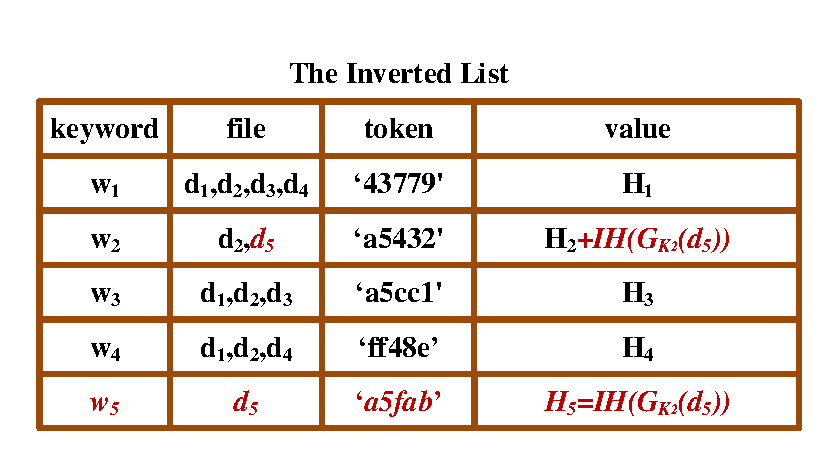
\includegraphics[width=5 in]{fig/inverted-index}
\DeclareGraphicsExtensions.
\caption{一个简单的倒排索引}
\label{fig:inverted-index}
\end{figure}

\begin{figure}[ht]
\centering
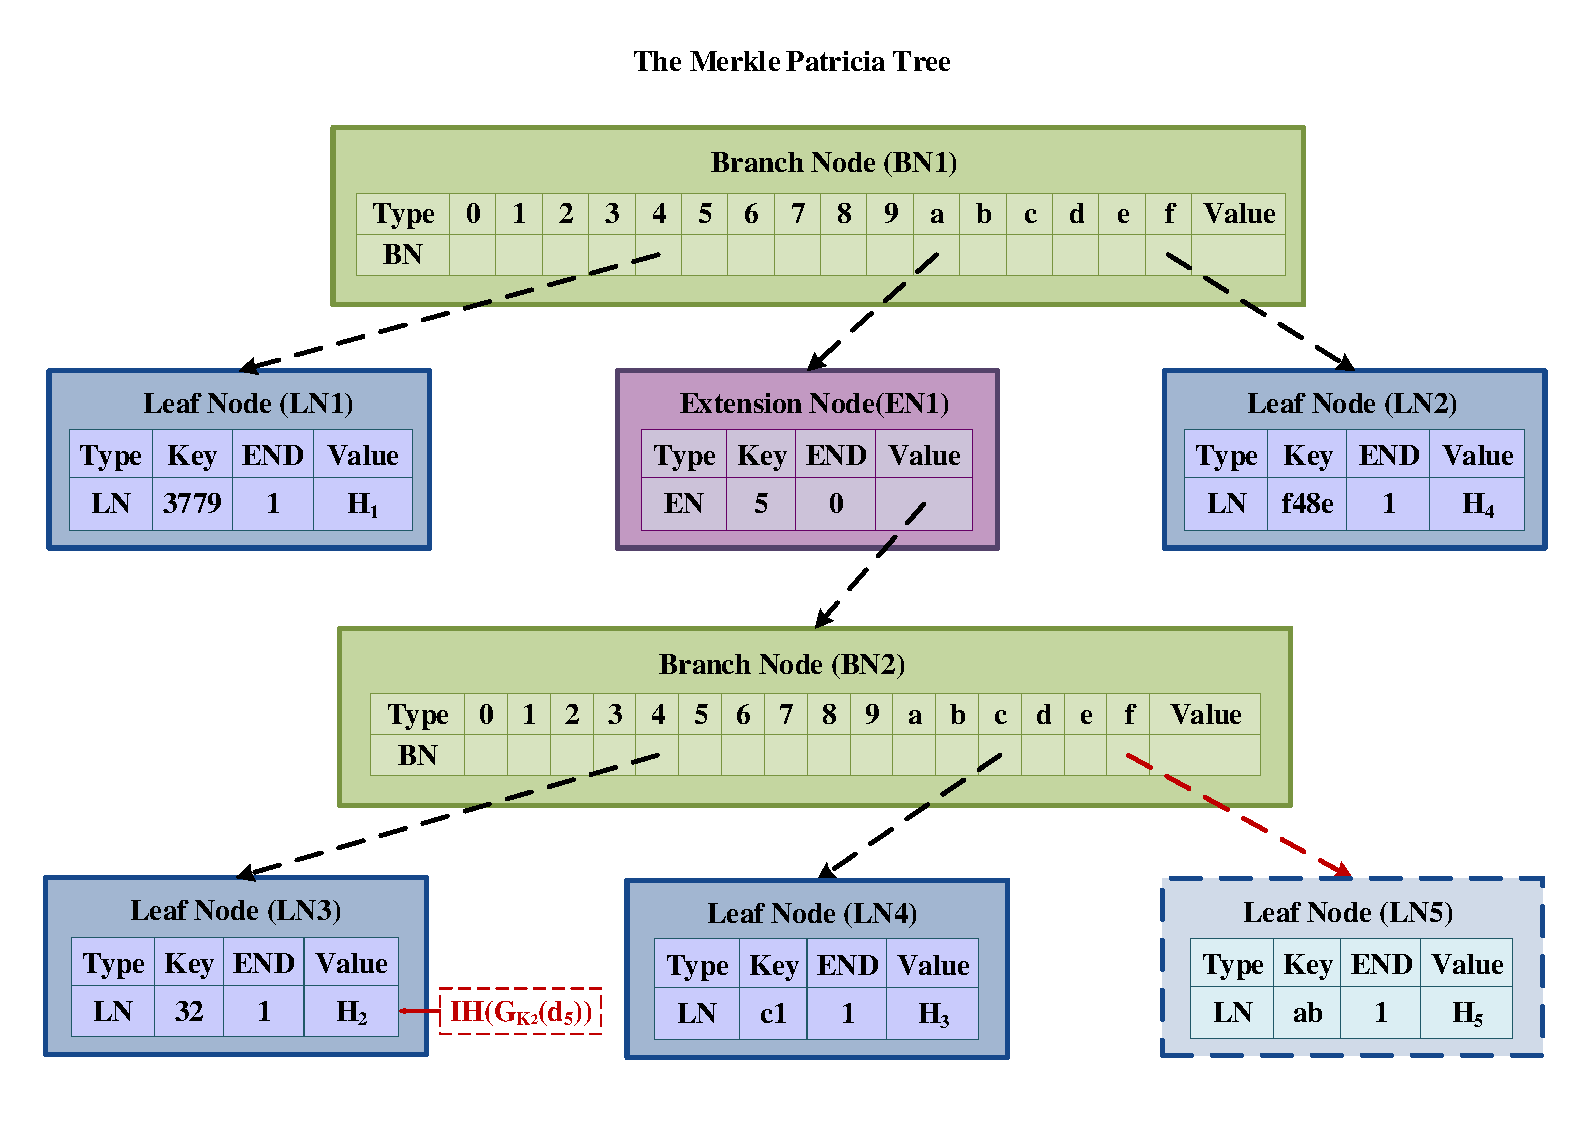
\includegraphics[width=6 in]{fig/MPT}
\DeclareGraphicsExtensions.
\caption{由倒排索引和MPT构建的验证索引}
\label{fig:MPT}
\end{figure}


\begin{figure}[ht]
  \begin{minipage}[b]{0.49\textwidth}
    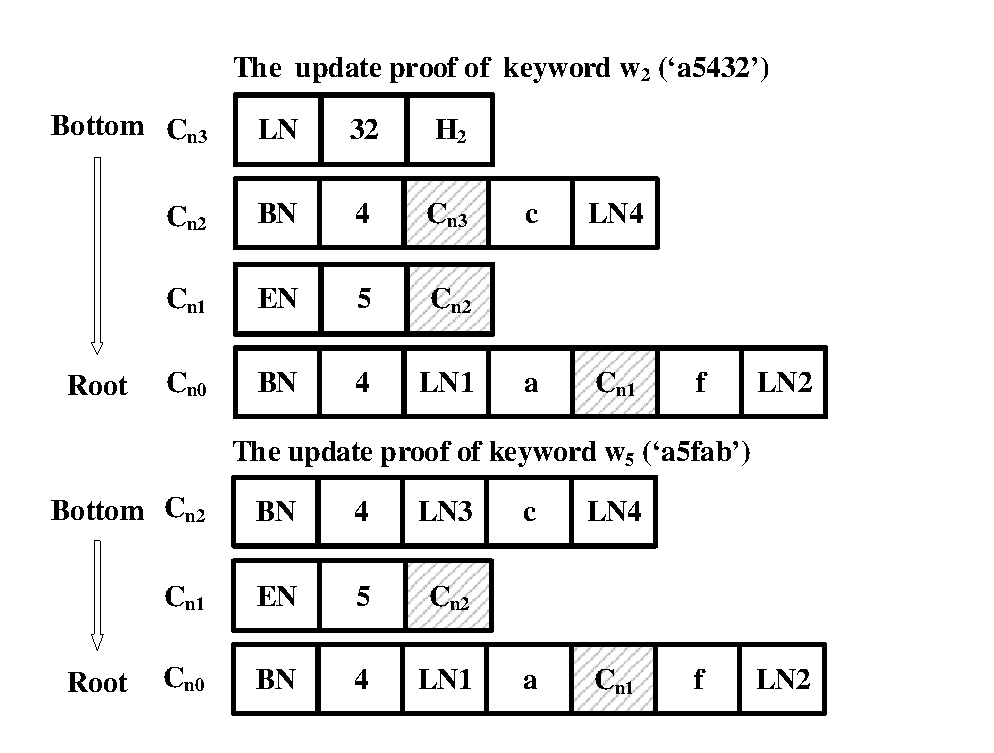
\includegraphics[width= 2.9 in]{fig/updateProof}
    \caption{更新证明}
    \label{fig:updateProof}
  \end{minipage}
  \begin{minipage}[b]{0.49\textwidth}
    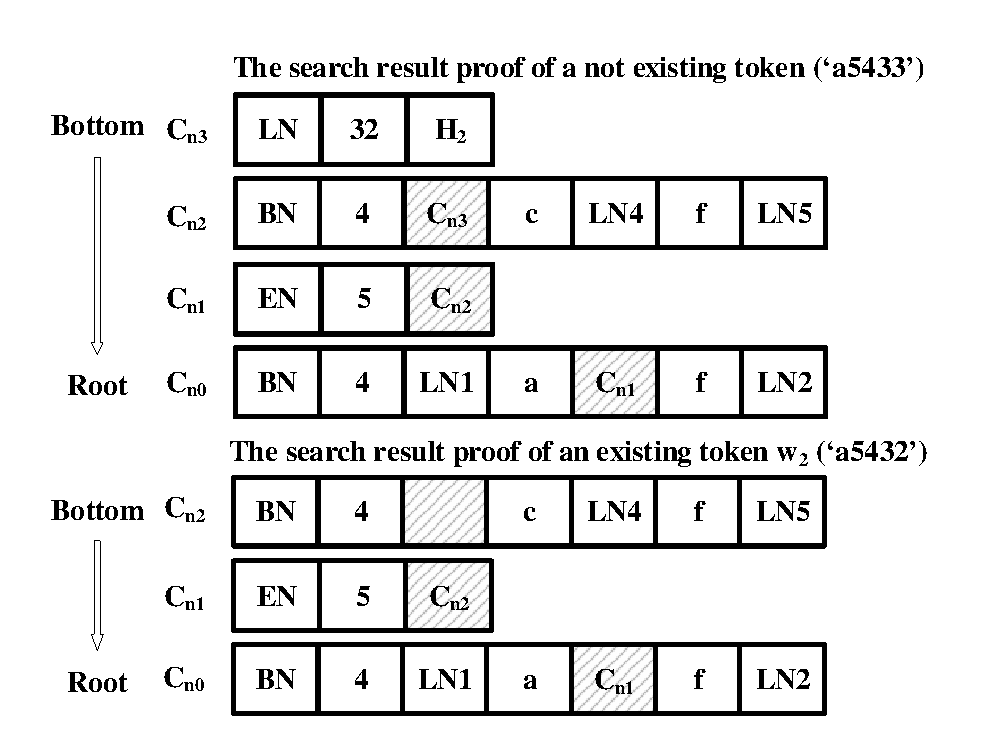
\includegraphics[width= 3.2 in]{fig/resultProof}
    \caption{结果证明}
    \label{fig:resultProof}
  \end{minipage}
\centering
\end{figure}

如图~\ref{fig:inverted-index},图\ref{fig:MPT},图\ref{fig:updateProof}和图\ref{fig:resultProof}所示,我们将通过一个解释性的实例来说明建立和更新验证索引$\lambda$,生成更新证明$\rho_u$和验证更新,以及生成结果证明$\rho_s$和验证搜索结果的过程。

{\heiti 建立并更新验证索引:}首先,我们假设数据持有者拥有四个文件,分别为$d_1,d_2,d_3,d_4$,他们包含了四个关键字$w_1,w_2,w_3,w_4$,其对应关系如图\ref{fig:inverted-index}中的倒排索引所示。由这四个文件构建的验证索引如图\ref{fig:MPT}所示。当包含关键字$w_2$和$w_5$的文件$d_5$新增时,对于已经存在的关键字$w_2$,云服务器只需将$IH(G_{K_2}(d_5))$添加到原有的叶子节点上。而对于不存在的关键字$w_5$,云服务器则需要创建一个新的叶子节点,并将$IH(G_{K_2}(D_5))$作为他的节点值。

{\heiti 生成更新证明和验证更新:}云服务器需要将两个涉及到更新的关键字$w_2$,$w_5$对应的路径返回给用户,用以作为更新证明$\rho_u$。如图~\ref{fig:updateProof}所示,当用户拿到该更新证明后,对于每一个待更新关键字,首先需要确保该关键字对应的令牌或其前缀出现在更新证明中,然后需要根据更新证明重构出根节点哈希,用于跟用户持有的根哈希进行对比。只有当每一个待更新关键字对应的更新证明重构出的根哈希与原根哈希相同时,更新验证才通过。验证通过后,用户通过更新令牌$\tau_u$和更新证明$\rho_u$构造出更新后的根哈希$rt'$,这确保了数据的新鲜性。

{\heiti 生成结果证明和验证搜索结果:}结果证明$\rho_s$的生成可以分为两种情况来讨论。
第一种情况,假设用户想要搜索的关键字为$w_2$,他提交的对应该关键字的挑战令牌为“a5432”。由于该关键字令牌在验证索引$\lambda$中已经存在,云服务器可以找到与该令牌对应的搜索路径{BN1,EN1,BN2,LN3},根据$Prove$算法,服务器会返回除$LN3$以外的路径上的“键值对”作为结果证明,如$C_{n2},C_{n1},C_{n0}$所示。用户在收到结果证明$C_{n2},C_{n1},C_{n0}$以后,可以根据该证明$\rho_s$和搜索结果$C_w$重新构建根哈希。具体过程如下:首先用户将令牌“a5432”与结果证明中$\rho_s$的“键”进行匹配,发现“a54”为令牌的前缀,因此剩余键$remain\_key$ 为“32”。随后用户根据“32”以及搜索结果$d_2,d_5$重新生成叶子节点$LN3$,并通过结果证明$\rho_s$自底向上构建冲根哈希的值。最后用户通过比较重构得到的根哈希和自身持有的根哈希,来判断数据是否完整。例如,假设云服务器只返回了文件$d_2$,那么重构得到的根哈希将与正确的根哈希不匹配。
第二种情况:假设用户搜索的关键字令牌为“a5433”,该令牌在验证索引$\lambda$中不存在。根据云服务器的查找方法,其搜索路径与“a5432”相同,但不同的是,该令牌在叶子节点$LN3$处发生了不匹配。因此云服务器需要从叶子节点$LN3$开始自底向上生成结果证明,如图~\ref{fig:resultProof}中的$C_n3,C_n2,C_n1,C_n0$所示。用户在收到该结果证明以后,由于发现搜索令牌$\tau_s$与结果证明$\rho_s$中的“键”无法匹配,因此$remain\_key$被置空。用户将直接根据结果证明$\rho_s$重构根哈希。同样,用户将其与正确的根哈希进行对比,如果不相同,则说明服务器篡改了搜索结果或是结果证明,产生了恶意行为。


\section{安全性分析}
在本节中,我们将对方案的安全性进行证明。方案的安全性主要分为两个部分,一个是机密性,另一个是可验证性。机密性是指敌手无法从验证索引$\lambda$和用户发送的令牌$\tau$中获取文件和关键字的明文信息。可验证性是指当服务器返回不完整或者错误的结果时,用户不会验证通过。
\begin{figure}[t]
\centering
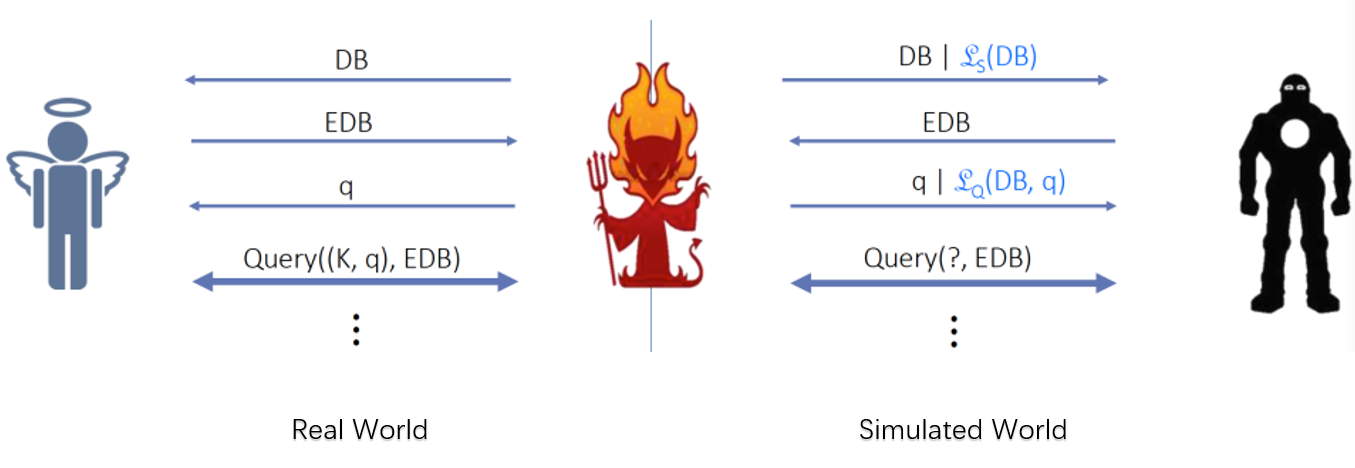
\includegraphics[width=6 in]{fig/security.png}
\DeclareGraphicsExtensions.
\caption{基于仿真博弈的安全性证明方案}
\label{fig:security}
\end{figure}

首先,我们采用基于仿真博弈 (Simulation-based Game)的安全性方案来证明方案的机密性。该方案的图形解释如图~\ref{fig:security}所示,我们需要确保一个敌手无法区分出$\mathbf{Real}$ World 和$\mathbf{Ideal}$ World 的输出。具体的定义如下:

\begin{definition}[\single 机密性]
  {\itshape
      令方案\single 是一个普适的、支持数据更新的可验证对称加密搜索方案,考虑以下概率性实验,其中 $\mathcal{A}$ 是一个有状态的敌手 (statefule adversary), $\mathcal{S}$ 是一个有状态的仿真者 (stateful simulator), $\mathcal{L}$ 是有状态的泄露函数 (leakage algorithms):

      $\mathbf{Real}_\mathcal{A}(k)$:一个挑战者采用$KGen(1^k)$生成了对称秘钥 $K_1,K_2$。敌手 $\mathcal{A}$ 选择了一个文件集 $\mathcal{D}$ 让挑战者通过 $\{\lambda\} \leftarrow Init(K_1,K_2,\mathcal{D})$ 算法生成验证索引 $\lambda$。同时,敌手 $\mathcal{A}$ 生成了多项式数量级的自适应查询 $q = \{w,f\}$。对于每一个查询 $q$, 敌手 $\mathcal{A}$ 从挑战者处收到一个搜索令牌 $\tau_w$ 和 更新令牌 $\tau_u$,其中 $\tau_w \leftarrow SearchToken(K_1,w)$,$(\tau_u) \leftarrow UpdateToken(K_1,K_2,f)$。最后,敌手 $\mathcal{A}$ 返回一个比特 $b$。

      $\mathbf{Ideal}_\mathcal{A,S}(k)$:一个敌手 $\mathcal{A}$ 选择了一个文件集 $\mathcal{D}$。 给定 $\mathcal{L}(\mathcal{D})$,仿真者 $\mathcal{S}$ 生成验证索引 $\lambda$ 发送给敌手 $\mathcal{A}$。敌手 $\mathcal{A}$ 生成了多项式数量级的自适应查询 $q = \{w,f\}$。对于每一个查询 $q$,仿真者 $\mathcal{S}$ 向其返回一个恰当的令牌 $\tau$。最后,敌手 $\mathcal{A}$ 返回一个比特 $b$。

      如果对于任何概率多项式时间 (Probabilistic Polynomial-Time, PPT)的敌手 $\mathcal{A}$, 始终存在一个概率多项式时间的仿真者 $\mathcal{S}$,使得,
      \begin{align}
        |Pr[\mathbf{Real}_A(k) = 1] - Pr[\mathbf{Ideal}_{A,S}(k) = 1]| \leq negl(k).
      \end{align}
      则我们认为 \single 是 $\mathcal{L}$-机密的。
  }
\end{definition}

在具体证明之前,我们首先给出敌手$\mathcal{A}$能看到的内容,即泄露函数$\mathcal{L}$的内容。$\mathcal{L}$ 定义如下:

\begin{align}
  \mathcal{L}(\mathcal{D})=(|\lambda|,{\tau}_q,{\sigma})
\end{align}

其中$|\lambda|$表示验证索引的大小,以叶子节点的数目来衡量。$\{\tau_q\}$表示由$q$个查询产生的令牌,$\sigma$表示验证索引中的搜索路径。我们有以下的定理:

\begin{theorem}
    如果$F$,$G$都是伪随机函数,那么方案\single 就是$\mathcal{L}$-机密的。
\end{theorem}

\begin{proof}
  我们将证明,对于任何概率多项式时间内的敌手$\mathcal{A}$,都存在一个概率多项式时间内的仿真者$\mathcal{S}$,使得真实游戏 $\mathbf{Real}_\mathcal{A}(k)$和仿真游戏 $\mathbf{Ideal}_\mathcal{A,S}(k)$在计算上是无法区分的 (computationally indistinguishable)。

  首先,给定$\mathcal{L}(\mathcal{D})=(|\lambda|,{\tau}_q,{\sigma})$,$\mathcal{S}$通过选择$|\lambda|$个随机“键值对”插入MPT中生成一个仿真的验证索引$\tilde{\lambda}$。由于在真实的验证索引中,“键值对”都是采用了伪随机函数$F$,$G$进行了伪随机化的,因此敌手$\mathcal{A}$将无法区分出真实的$\lambda$和仿真的$\tilde{\lambda}$。

  模拟搜索令牌时,对于第一个令牌 $\tau_w$ ,如果它与 $\{\sigma\}$ 中的某一路径匹配,那么 $\mathcal{S}$ 就在 $\tilde{\lambda}$ 中选择任意一条路径作为令牌 $\tilde{\tau_w}$ 发送给敌手 $\mathcal{A}$,否则 $\mathcal{S}$ 就选择不在 $\tilde{\lambda}$ ̃路径中的随机字符串作为令牌 $\tilde{\tau_w}$ 发送给敌手 $\mathcal{A}$。对于后续的令牌,如果 $w$ 之前出现过,那么令牌 $\tilde{\tau_w}$ ̃就和之前发送给敌手 $\mathcal{A}$的维持一样。如果 $w$ 没出现过,那么令牌的生成方式就和第一个令牌的生成方式一样。由于令牌采用了伪随机函数$F$进行了加密,因此敌手$\mathcal{A}$也无法区分真实的令牌和仿真的令牌。

  模拟更新令牌时,更新令牌被设置为$\tilde{\tau_u} = (\tilde{\tau_{w_1}},\cdots,\tilde{\tau_{w_{|W_d|}}},\tilde{\tau_r})$。对每一个更新令牌$\tilde{\tau_{w_i}}$,其中$i \in \{1,\cdots, |W_d|\}$,$\mathcal{S}$ 的模拟方法与模拟搜索令牌方法相同。由于每一个更新令牌都采用了伪随机函数$F$进行了加密,并且文件$d$采用了伪随机函数$G$进行了加密,因此敌手 $\mathcal{A}$ 无法区分真实的令牌、文件与仿真的令牌、文件。

  因此我们可以得到结论:真实实验$\mathbf{Real}_\mathcal{A}(k)$和仿真实验$\mathbf{Ideal}_\mathcal{A,S}(k)$的输出结果是不可区分的。
\end{proof}

\single 方案的可验证性意味着该方案可以验证数据的新鲜性和完整性,即防御定义~\ref{def:freshness}和~\ref{def:integrity}提出的两种攻击。这里我们采用了一个基于游戏 (game-based)的安全性定义来证明\single 方案的可验证性。

\begin{definition}[\single 可验证性]
  \itshape{
      令方案\single 是一个普适的、支持数据更新的可验证对称加密搜索方案,考虑以下概率性实验,其中 $\mathcal{A}$ 是一个有状态的敌手 (statefule adversary):

      \noindent$\mathbf{Vrf}_\mathcal{A}(k)$:
      \begin{enumerate}[1.]
        \item 挑战者通过 $KGen(1^k)$ 生成对称秘钥 $K_1,K_2$。
        \item 敌手 $\mathcal{A}$ 给挑战者选择一个文件集合 $\mathcal{D}$。
        \item 挑战者通过$\{\lambda\} \leftarrow Init(K_1,K_2,\mathcal{D})$生成一个验证索引 $\lambda$。
        \item 给定 $\lambda$ 和 对算法 $SearchToken(K_1,w)$, $UpdateToken(K_1,K_2,d)$ 的预言权限, 敌手 $\mathcal{A}$ 输出一个关键字令牌 $\tau_w'$, 和一系列加密文件 $C'$,其中 $C' \neq C_w$,同时输出%更新证明 $\rho_u'$ 和
        结果证明$\rho_s'$.
        \item 挑战者计算 $b:=Verify(K_1,K_2,C',\rho_s',\tau_w')$.
        \item 实验的输出为一个比特 $b$.
      \end{enumerate}
      如果对于任何概率多项式时间 (Probabilistic Polynomial-Time, PPT)的敌手 $\mathcal{A}$,
      \begin{align}
        Pr[\mathbf{Vrf}_\mathcal{A}(k)=1] \leq negl(k).
      \end{align}
      成立,则我们认为\single 方案是可验证的。
  }
\end{definition}

\begin{theorem}
    如果哈希函数$H$和增量哈希函数$IH$是抗碰撞的,并且$G$是伪随机函数,那么\single 方案就是可验证的。
\end{theorem}

\begin{proof}
  考虑服务器返回的搜索结果为$\tilde{D_w}$,而正确的搜索结果为$D_w$,其中$\tilde{D_w} \neq D_w$。但是用户的$Verify$算法通过了$\tilde{D_w}$作为正确搜索结果的情况。对于$Verify$算法,这种情况的产生存在两种可能。第一种是在计算$\tilde{D_w}$ ̃和$D_w$对应的伪随机值和增量哈希值时产生了碰撞,第二种是在生成根哈希的路径中产生了哈希碰撞。不管是哪一种,都可以推出哈希函数产生了碰撞或者伪随机函数产生了碰撞,但是哈希函数产生碰撞或者伪随机函数产生碰撞的可能性是小于一个可忽略的值的,因此,我们的方案是可验证的。
\end{proof}


\section{实验结果}

\begin{figure}[bhpt]
\centering
  \begin{minipage}[b]{0.48 \textwidth}
    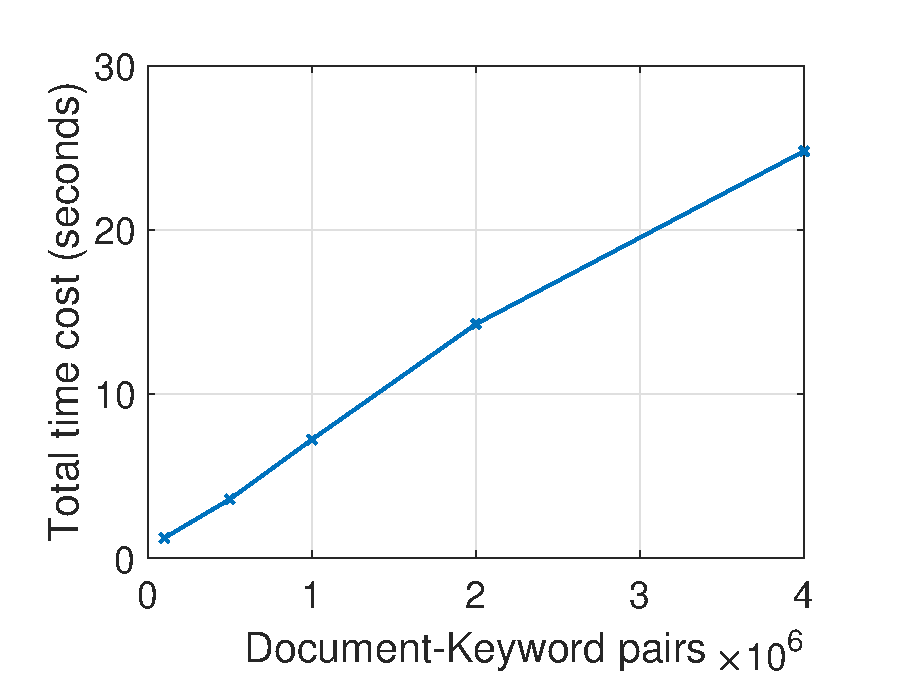
\includegraphics[width=\textwidth]{expr/initialization}
    \caption{$Init$ delays}
    \label{fig:init}
  \end{minipage}
  \begin{minipage}[b]{0.48 \textwidth}
    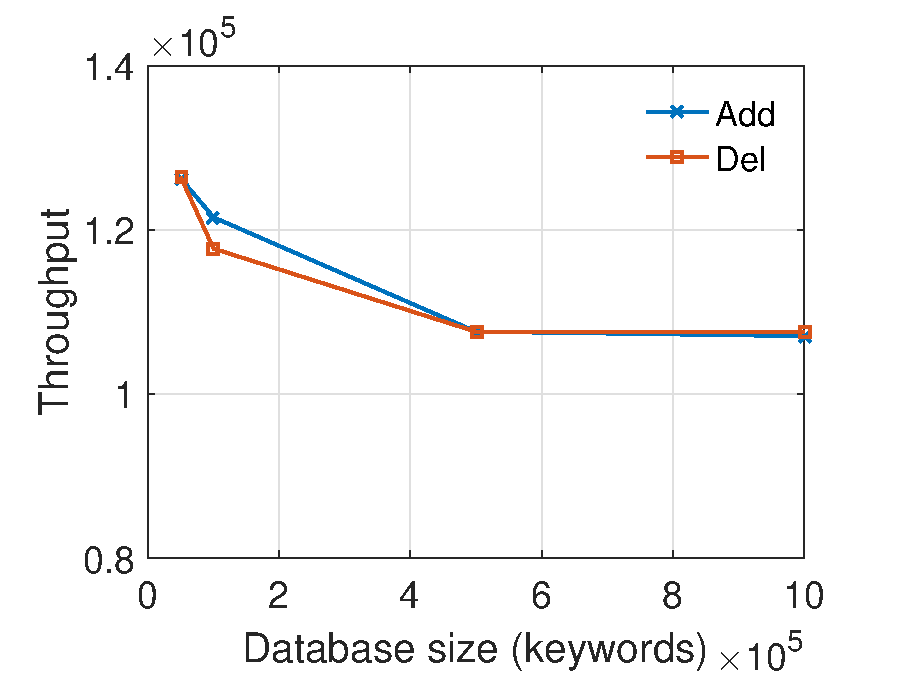
\includegraphics[width=\textwidth]{expr/update}
    \caption{$PreUpdate$ throughput}
    \label{fig:update}
  \end{minipage}

  \hspace{-40.0pt}
  \par \vspace{-10.pt}
  \hspace{-36.0pt}

  \begin{minipage}[b]{0.48 \textwidth}
    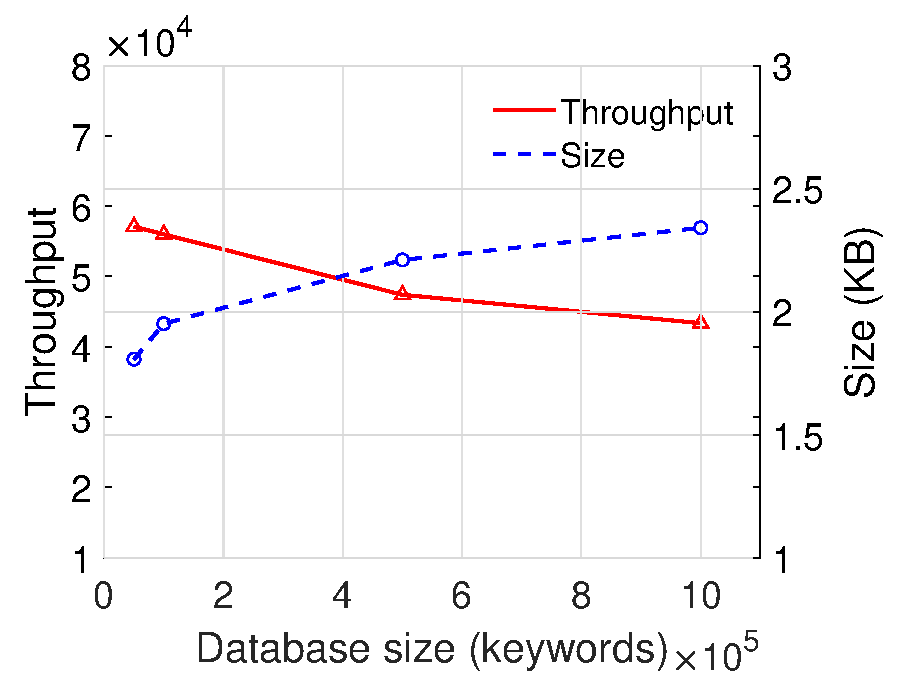
\includegraphics[width=\textwidth]{expr/prove}
    \caption{$Prove$ cost}
    \label{fig:prove}
  \end{minipage}
  \begin{minipage}[b]{0.48 \textwidth}
    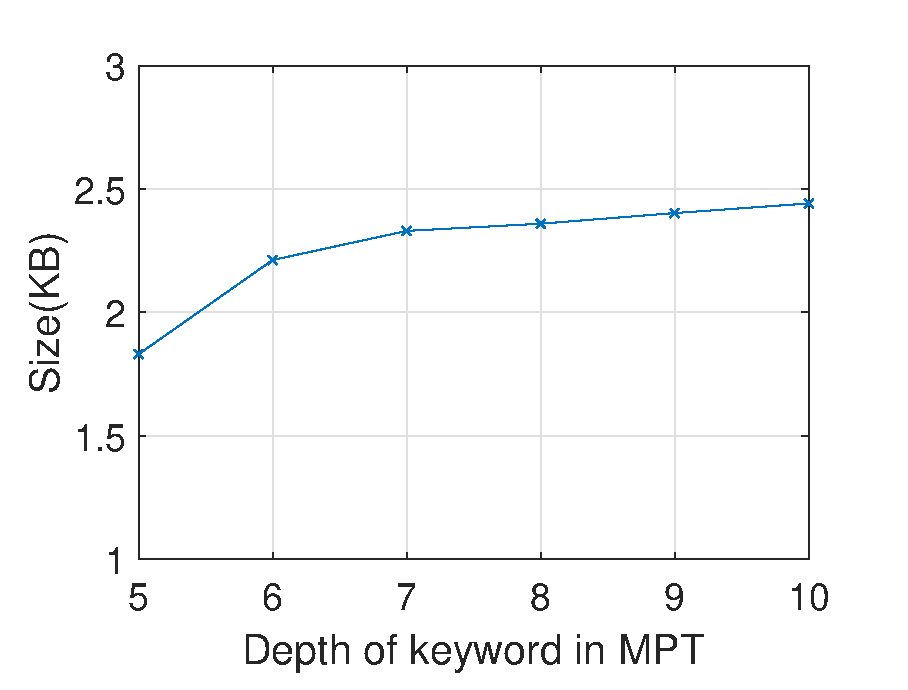
\includegraphics[width=\textwidth]{expr/proof}
    \caption{Proof cost of MPT}
    \label{fig:proof}
  \end{minipage}

  \hspace{-40.0pt}
  \par \vspace{-10.pt}
  \hspace{-36.0pt}

  \begin{minipage}[b]{0.48 \textwidth}
    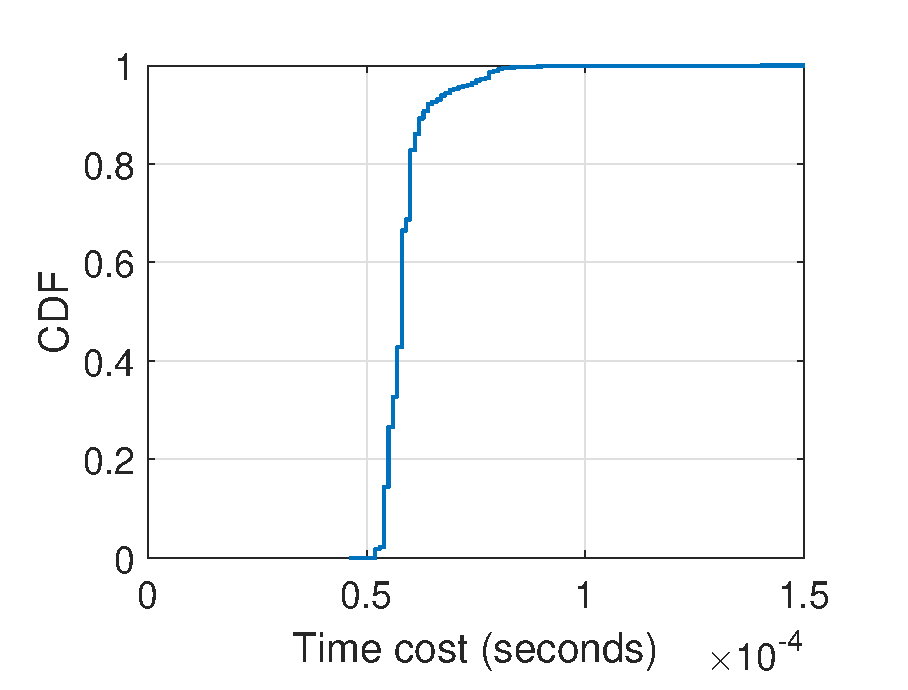
\includegraphics[width=\textwidth]{expr/verify}
    \caption{$Verify$ performance}
    \label{fig:verify}
  \end{minipage}
  \begin{minipage}[b]{0.48 \textwidth}
    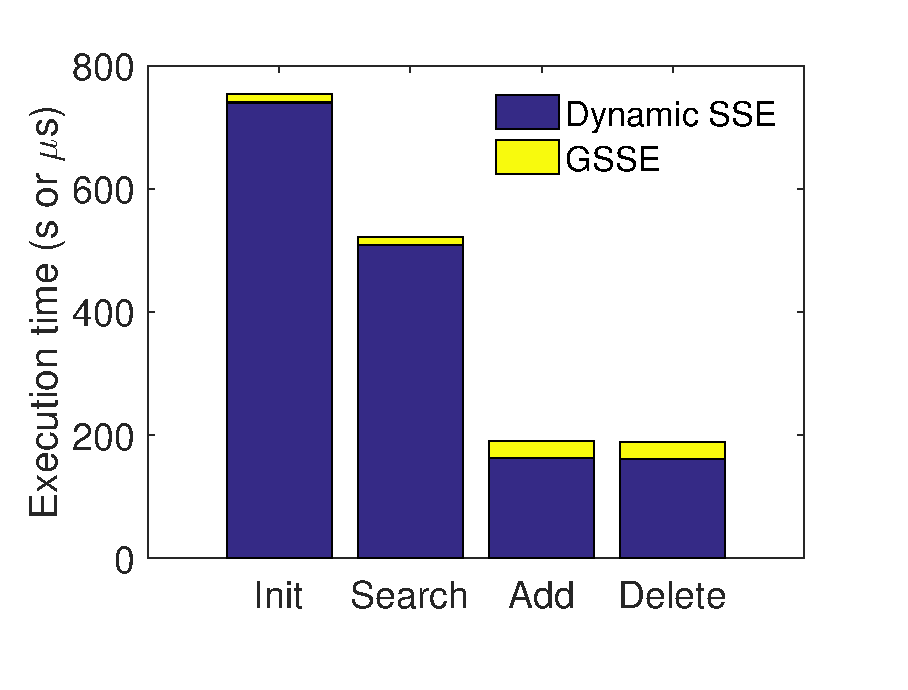
\includegraphics[width=\textwidth]{expr/comparison}
    \caption{Comparison with SSE~\cite{cash2014dynamic}}
    \label{fig:comparison}
  \end{minipage}
\centering
\end{figure}

\subsection{实验设置}
为了证明方案\single 的有效性,我们通过 Crypto++ 5.6.5 库实现了方案的原型。原型系统包含大约2200行代码。我们使用 HMAC-SHA256 作为两个随机预言 (random-oracle),使用 SHA3-256 作为哈希函数,使用 MuHash 作为增量哈希函数。我们的实验在一台处理器为 Intel Core i5 2.5GHz,内存为 4G 的笔记本上进行,使用单线程实现。

我们使用一个开源数据集Enron email dataset~\cite{enron_email}作为实验的测试数据集,使用了其中从“allen-p”到“kaminski-v”之间的数据。我们从该数据集中提取出了大量的“文件-关键字”对 (document-keyword pairs),并通过python脚本为他们构建出了明文的倒排索引。注意,从文件中提取关键字的时延并没有被考虑在实验评估中,因为该问题与我们研究的\single 方案是一个独立的问题。

下文中,我们首先评估了\single 方案的算法效率,然后将\single 方案与一个著名的对称加密搜索方案~\cite{cash2014dynamic}进行了结合,以此来证明\single 方案引入的结果验证的开销并不大。注意,如无特别说明,下文中的每一个实验结果都是十次实验的平均值。


\subsection{实验结果}
首先,我们评估了$Init$算法的时延,即数据持有者生成验证索引$\lambda$所需的时间。如图~\ref{fig:init}所示,生成验证索引$\lambda$所需的时间与“文件-关键字”对的数量大小成正比,因为向MPT中执行的插入操作与“文件-关键字”对的数量相同。总体来说,$Init$ 算法在 “文件-关键字”对达到400万的时候,可以在25秒内执行完毕。由于$Init$算法仅需要在初始化时执行一次,因此这个开销是可以接受的。

%The delays of generating the proof index are proportional to the size of the document-keyword pairs, since \name performs the same number of insertions to the number of the document-keyword pairs. Overall, the initialization consumes around 25 seconds where the documents include four million keywords, which is acceptable.
% for the initialization process.
云服务器更新验证索引的时间如图~\ref{fig:update}所示,更新的时延与数据库的大小有关,即与验证索引的大小有关,而验证索引的大小由它包含的关键字数量来衡量。严格意义上来书,一次更新的时延与MPT树的层数有关。为了更好的展示更新时延与验证索引大小的关系,我们使用了大量的关键字来评估更新时延。由于每一个文件包含的关键字个数不同,这里我们采用吞吐量(throughput)来衡量每秒钟云服务器可以更新的“文件-关键字”对。从图中可以看到,$Add$和$Del$操作的性能几乎相同。当数据库的大小增大时,吞吐量将会降低。当数据库的大小为100万个关键字时,云服务器每秒钟可以同时支持110,000此更新操作。同时,我们也测量了用户端$UpdateToken$算法引入的带宽开销,更新令牌$\tau_u$中每一个关键字对应的密文带来的平均开销大小在 32字节左右,而更新令牌的总大小与待更新文件$d$包含的关键字个数有关,这也是可以接受的。


如图~\ref{fig:prove}所示,云服务器可以在数据库大小在100万关键字时,每秒钟进行43,000次 $Prove$ 操作,这意味着云服务器可以同时支持43,000个来自用户的查询请求。由$Prove$操作产生的结果证明$\rho_s$的大小也可以在图~\ref{fig:prove}和图~\ref{fig:proof}中看到,结果证明的大小随着MPT层数的增加而增长,但总体而言,只需要几千字节。

我们通过累计分布函数图 (Cumulative Distribution Function, CDF)来对用户端进行的$Verify$操作进行了测试。结果显示,几乎99.7\%的情况下,用户端都可以在0.1毫秒内完成结果验证,这是可以接受的。

除此以外,我们还对MPT的存储空间进行了评估。如果我们使用一个100万个关键字的数据库,MPT的存储空间大小大约为82MB,而该数据库本身所占用的空间大小为 590MB,因此MPT带来的额外存储开销不算特别大。特别需要说明的是,这里我们评估数据库大小所采用为关键字密集型的数据,即邮件数据。如果数据持有者需要加密的是媒体类型的数据,例如图片或是音乐文件等等,这些文件只包含少量的关键字和属性,因此为这些类型的数据构建验证索引时,验证索引占原数据集的比例将会很小,甚至可以忽略。



\subsection{与SSE方案的对比}

我们将我们的普适性可验证对称加密搜索方案\single ,与Cash等人提出的一个较为知名的动态对称加密搜索方案 (Dynamic Symmetric Searchable Encryption, DSSE)~\cite{cash2014dynamic}进行了结合,并展示了\single 为其提供结果验证服务带来的额外开销并不大。

为了公平的进行性能比较,我们使用了同样的数据集,并在同样的设备参数下对两个方案联合进行了实验。如图~\ref{fig:comparison}所示,我们测量了$Init$阶段,$Search$阶段和$PreUpdate$阶段的性能开销。图中,$Init$操作使用了200万个“文件-关键字”来分别构建DSSE方案~\cite{cash2014dynamic}和方案\single 用到的索引,时间单位为秒。而其他三个操作$Search, Add, Delete$的评估采用的数据库大小为10,000个关键字,时间单位为微妙。注意,DSSE方案~\cite{cash2014dynamic}中的$Search$操作与\single 方案中的$Prove$操作对应。从图中可以看出,我们的\single 方案引入的额外开销非常小。其中,相较于DSSE方案~\cite{cash2014dynamic}而言,方案\single 在$Init$阶段引入的开销非常小,仅仅额外引入了1.9\%的额外开销。而对于一次$Search$ ($Prove$) 操作来说,\single 方案给云服务器引入的额外开销为14微秒,仅仅给DSSE方案带来了2\%的额外开销。同样的,对于一次$Add$或$Delete$操作来说,我们的\single 方案仅仅引入了27微秒的时间,仅占方案~\cite{cash2014dynamic}的 17\%。

在表~\ref{tab:compareSSE}中,我们还比较了二者的通信开销。由于数据的方差较大,每一个实验结果都是50,000次实验的平均值。结果显示,DSSE方案~\cite{cash2014dynamic}的搜索结果大小平均为53KB左右,而我们的结果证明大小仅仅为3KB左右,即由\single 方案引入的额外开销低于6\%。此外,DSSE方案~\cite{cash2014dynamic}生成的令牌大小平均为390B,而\single 方案生成的令牌仅为32B,即由\single 方案引入的额外开销低于9\%。这些实验结果充分表明了,\single 方案是实用且高效的。



\begin{table}[h]
  \begin{center}
  \caption{Comparison with the SSE scheme proposed by Cash et al.~\cite{cash2014dynamic}}
  \label{tab:compareSSE}
  %\begin{threeparttable}
  \begin{tabular}{|c|c|c|}
    \hline
    Communication cost   & SSE~\cite{cash2014dynamic} &\single          \\
    \hline
    Search token          & 390 Bytes                 & 32 Bytes       \\
    \hline
    Search result/proof   & 53 Kilobytes              & 3 Kilobytes          \\
    \hline
  \end{tabular}
\end{center}
\end{table}
